%\begin{center}
%\large \bf \runtitulo
%\end{center}
%\vspace{1cm}
\chapter{Práctico Tema 4}

1. AbueloOAbuela $\equiv$ Persona $\sqcap$ $\exists$hijo-de.PadreOMadre\\ 

AbuelaMaterna $\equiv$ Mujer $\sqcap$ AbueloOAbuela\\


PadreOMadreDeMasDeDos $\equiv$ Persona $\sqcap >= $2 (hijo-de.Persona)\\

HermanoOHermana $\equiv \exists$hijo-de$^-1$.PadreOMadreDeMasDeDos\\

SinHijos $\equiv$ Persona $\sqcap$ $\neg \exists$hijo-de.Persona\\

TioTia $\equiv$ Persona $\sqcap$ HermanoOHermana $\sqcap \exists$hijo-de$^-1$.AbueloOAbuela\\

TioSinHijos $\equiv$ TioTia $\sqcap$ SinHijos\\


AbueloOAbuelaDeMasDeDos $\equiv$ PadreOMadreDeMasDeDos $\sqcap$ AbueloOAbuela\\

PadreDelSobrinoDeUnaNuera $\equiv \exists$ hijo-de$^-1$.AbueloOAbuelaDeMasDeDos \\

SobrinoDeUnaNuera $\equiv$ Hombre $\sqcap$ $\exists$hijo-de$^-1$.(PadreDelSobrinoDeUnaNuera)\\


PadreConAlMenos3HijosDosMujeres $\equiv$ Persona $\sqcap >=$3 (hijo-de.Persona) $\sqcap >=$2 (hijo-de.Mujer)\\



2. Teniendo el siguiente programa en Datalog: \\

\begin{enumerate}
	\item $father(alice, bob).$
	\item $mother(alice, carla).$
	\item $mother(evan, carla).$
	\item $father(carla, david).$

	\item $parent(X, Y) \gets father(X, Y)$
	\item $parent(X, Y) \gets mother(X, Y)$
	\item $ancestor(X, Y) \gets parent(X, Y)$
	\item $ancestor(X,Z) \gets parent(X, Y) \land ancestor(Y, Z)$
\end{enumerate}

Para derivar $parent(evan, david)$ uno debe apoyarse en las reglas 5 y 6 sería necesario que $father(evan, david).$ o $father(evan, david).$ existieran. Como no es el caso, $parent(evan, david)$ no se puede derivar. \\

Para el caso de $ancestro(carla, david)$, si es posible la derivación. A continuación, se presenta el árbol: \\

\begin{center}
	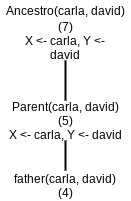
\includegraphics[]{Images/guia4ejercicio2.png}
	\captionof{figure}{Árbol de derivación}
	\label{fig:overview}
\end{center}



3. Dada la consulta conjunctiva: Q(X,Y) = $\exists$Z.parent (X,Y) $\bigwedge$ parent (Z,Y) ¿Qué regla debemos agregarle a P (slide 49)? ¿Cual sería el conjunto de respuesta? Verifiquelo en ABCDatalog.\\

Debemos agregar la regla:\\

$Q(X, Y) \gets parent(X, Y) \land parent(Z, Y).$\\

Este es el resultado de la consulta Q(X, Y) sería el equivalente a $parent(X, Y)$; en ABCDatalog: \\

$\{Q(alice, bob), Q(alice, carla), Q(carla, david), Q(evan, carla)\}$ \\

4. $Q_{1} \gets parent(X, Y) \land parent(Z, Y).$\\



5. De esta forma queda el mundo de bloques modelado en Datalog: \\

$estaSobre(b, a).$\\

$tresBloques(a).$
$tresBloques(b).$
$tresBloques(c).$\\

$estaSobreTresBloques(X, Y) \gets tresBloques(X), tresBloques(Y), X != Y, estaSobre(X, Y).$ \\

$estaSobreMesa(X) \gets tresBloques(X), tresBloques(Y), tresBloques(Z), X != Y,  X != Z, Y != Z, not estaSobre(X, Y), not estaSobre(X, Z).$\\

$estaApiladoSobre(X, Y) \gets estaApiladoSobreInmediatamente(X, Y).
estaApiladoSobre(X, Y) \gets estaApiladoSobre(X, Z), estaApiladoSobre(Z, Y).$\\

$estaDebajo(X, Y) \gets estaApiladoSobre(Y, X).$\\

$estaApiladoSobreInmediatamente(X, Y) \gets estaSobreTresBloques(X, Y).$\\

$estaDebajoInmediatamente(X, Y) \gets estaSobreTresBloques(Y, X).$\\

$puedeDesapilar(X) \gets tresBloques(X), tresBloques(Y), tresBloques(Z), X != Y,  X != Z, Y != Z, not estaSobreMesa(X), not estaSobre(Y, X), not estaSobre(Z, X).$\\

6. Proponga un ejemplo de dos esquemas de bases de datos (fuente y destino), muestre las s-t-TGDs necesarias para pasar de uno a otro, similar a slide 91, explique la transformación necesaria. Defina una instancia de bases de datos en el esquema fuente y muestre cual seria la solución (la instancia destino) para el problema de intercambio de datos. \\

\bigskip